% \documentclass[aspectratio=169,notes]{beamer}
\documentclass[aspectratio=169]{beamer}
\usetheme[faculty=phil]{fibeamer}
\usepackage{polyglossia}
\setmainlanguage{english} %% main locale instead of `english`, you
%% can typeset the presentation in either Czech or Slovak,
%% respectively.
\setotherlanguages{russian} %% The additional keys allow
%%
%%   \begin{otherlanguage}{czech}   ... \end{otherlanguage}
%%   \begin{otherlanguage}{slovak}  ... \end{otherlanguage}
%%
%% These macros specify information about the presentation
\title[Theoretical Mechanics]{Theoretical Mechanics, Lab 10: DYN ANGULAR} %% that will be typeset on the
\subtitle{Theorem on the: \\
Change of Principal Angular momentum of a system \\ \ } %% title page.
\author{Oleg Bulichev}
%% These additional packages are used within the document:
\usepackage{ragged2e}  % `\justifying` text
\usepackage{booktabs}  % Tables
\usepackage{tabularx}
\usepackage{tikz}      % Diagrams
\usetikzlibrary{calc, shapes, backgrounds}
\usepackage{amsmath, amssymb}
\usepackage{url}       % `\url`s
\usepackage{listings}  % Code listings
% \usepackage{subfigure}
\usepackage{floatrow}
\usepackage{subcaption}
\usepackage{mathtools}
\usepackage{todonotes}
\usepackage{fontspec}
\usepackage{multicol}
\usepackage{pdfpages}
\usepackage{wrapfig}
\usepackage{animate}
\usepackage{booktabs}
\usepackage{multirow}
% \usepackage{graphicx}
\usepackage{colortbl}
\usepackage{catchfilebetweentags}
\usepackage{makecell}
\graphicspath{{resources/}}
\frenchspacing

\setbeamertemplate{caption}[numbered]
\usetikzlibrary{graphs}

% \usepackage[backend=biber,style=ieee,autocite=footnote]{biblatex}
% \addbibresource{biblio.bib}
% \DefineBibliographyStrings{english}{%
%   bibliography = {References},}

\newcommand{\oleg}[2][] {\todo[color=red, #1] {OLEG:\\ #2}}
\newcommand{\fbckg}[1]{\usebackgroundtemplate{\includegraphics[width=\paperwidth]{#1}}}%frame background

\usepackage[framemethod=TikZ]{mdframed}
\newcommand{\dbox}[1]{
\begin{mdframed}[roundcorner=3pt, backgroundcolor=yellow, linewidth=0]
\vspace{1mm}
{#1}
\vspace{1mm}
\end{mdframed}
}

\begin{document}
\setlength{\abovedisplayskip}{0pt}
\setlength{\belowdisplayskip}{0pt}
\setlength{\abovedisplayshortskip}{0pt}
\setlength{\belowdisplayshortskip}{0pt}

\fbckg{fibeamer/figs/title_page.png}
\frame[c]{\setcounter{framenumber}{0}
    \usebeamerfont{title}%
    \usebeamercolor[fg]{title}%
    \begin{minipage}[b][6.5\baselineskip][b]{\textwidth}%
        \textcolor{black}{\raggedright\inserttitle}
    \end{minipage}
    % \vskip-1.5\baselineskip

    \usebeamerfont{subtitle}%
    \usebeamercolor[fg]{framesubtitle}%
    \begin{minipage}[b][3\baselineskip][b]{\textwidth}
        \raggedright%
        \insertsubtitle%
    \end{minipage}
    \vskip.25\baselineskip
}
%   \frame[c]{\maketitle}

\fbckg{fibeamer/figs/common.png}


\section*{Theory}

\begin{frame}[t]{Difference between torque and moment}
    \framesubtitle{}
    \begin{minipage}{0.8\textwidth}
        In Theoretical mechanics (we are operating with absolute rigid 
        bodies) — it’s the same. \\
        In Strength of materials — it different. Torque - twisting moment, 
        moment - Bending moment \\
    \end{minipage}
    \end{frame}
    
    \begin{frame}[t]{Moment (torque)}
    \framesubtitle{}
        \vspace{-0.6cm}
        \begin{figure}[H]
            \centering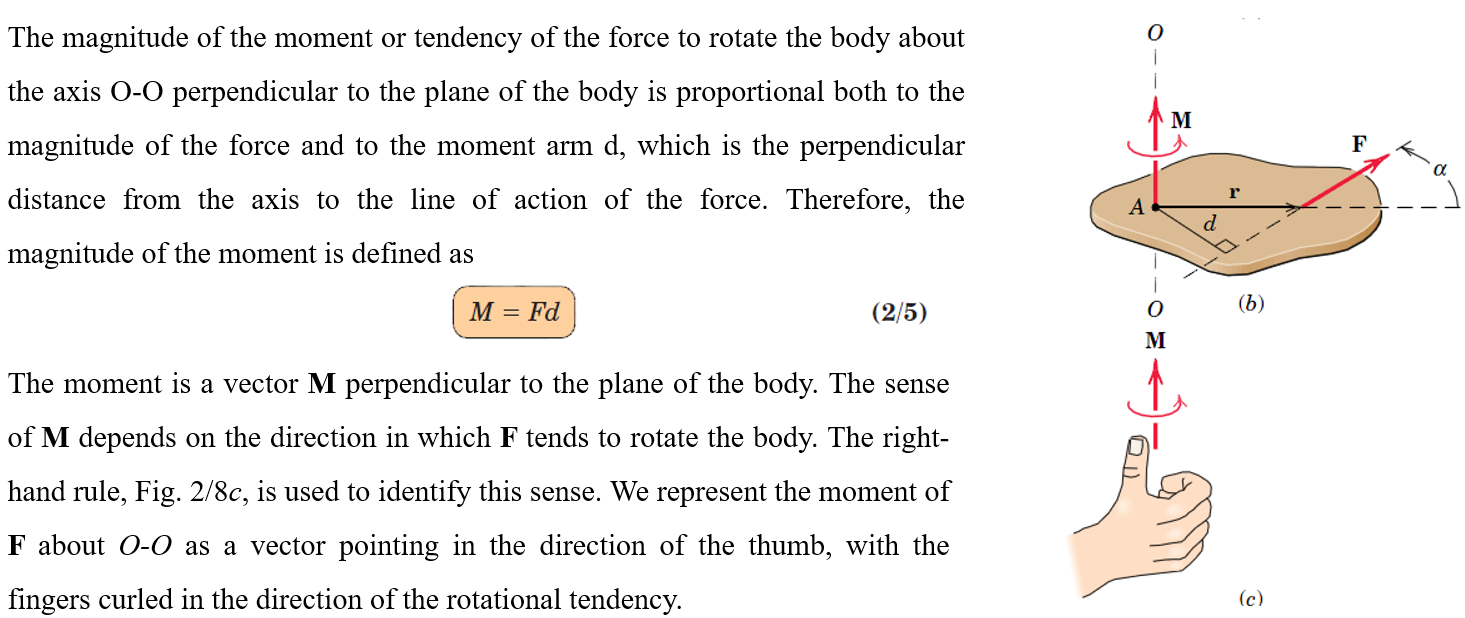
\includegraphics[height=6cm,width=1\textwidth,keepaspectratio]{image14.png}
            \label{fig:image14}
        \end{figure}
    \end{frame}
    
    \begin{frame}[t]{Torque and couple - intuitive explanation}
    \framesubtitle{}
        \begin{minipage}{0.8\textwidth}
            \textbf{Torque} is a value that shows the possibility of force to 
            rotate the body
            \begin{itemize}
                \item It’s not real thing (force is real), it’s math technique. 
                It is the reason why torque value depends on point 
                which we are using to calculate.
            \end{itemize}
            \textbf{Couple} — special case of torque, when it’s appears 
            because of two parallel forces (more info on next slide). 
            It has some unique properties (doesn’t depend on the 
            point of calculation).
        \end{minipage}
    \end{frame}
    
    \begin{frame}[t]{Couple}
    \framesubtitle{}
        \vspace{-0.6cm}
        \begin{figure}[H]
            \centering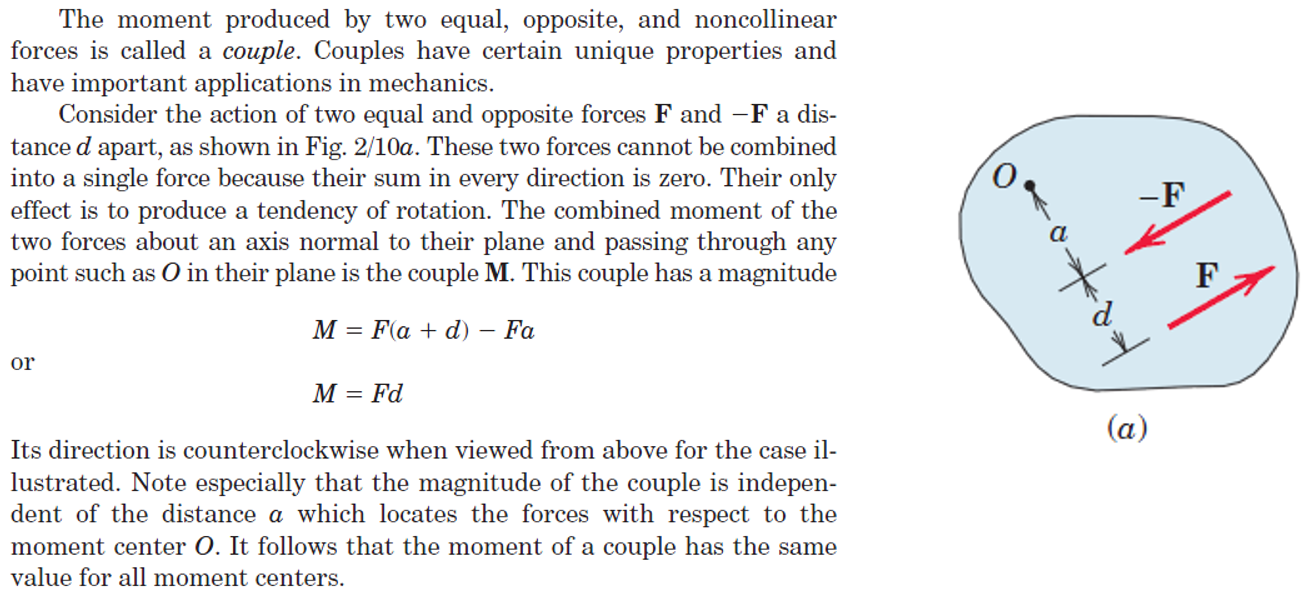
\includegraphics[height=6cm,width=1\textwidth,keepaspectratio]{image8.png}
            \label{fig:image8}
        \end{figure}
    \end{frame}
    
    \begin{frame}[t]{Force-Couple System    }
    \framesubtitle{}
        \vspace{-0.6cm}
        \begin{figure}[H]
            \centering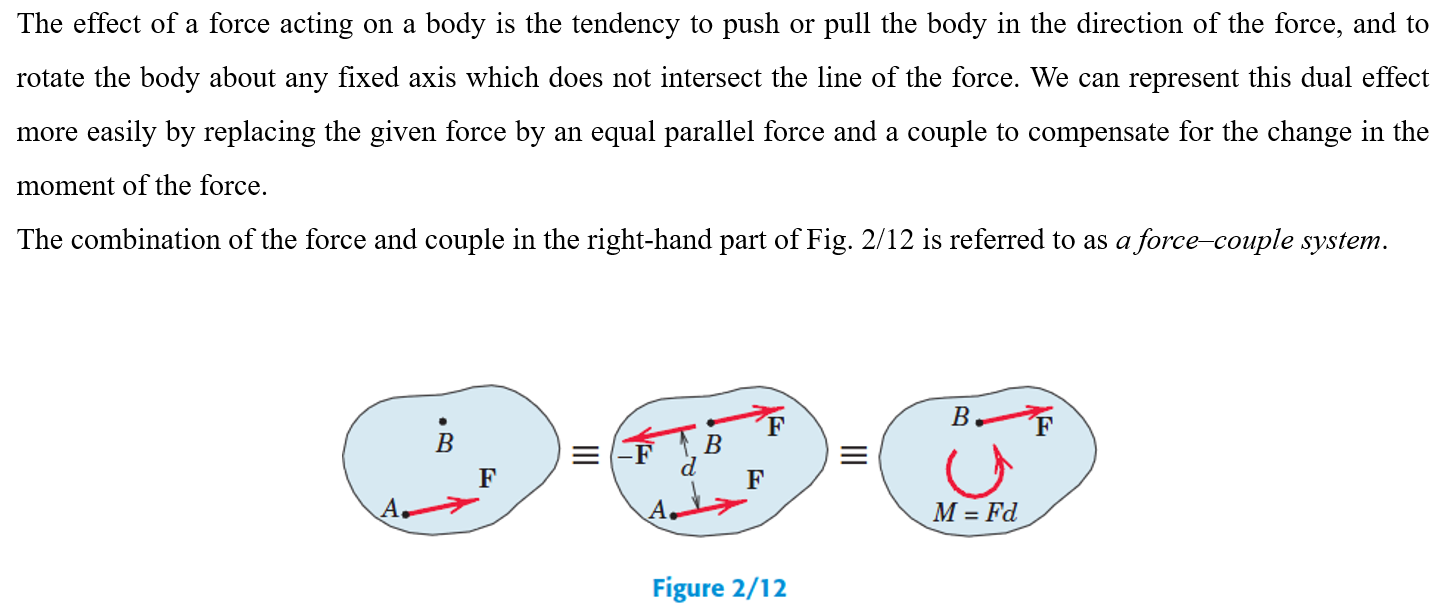
\includegraphics[height=6cm,width=1\textwidth,keepaspectratio]{image13.png}
            \label{fig:image13}
        \end{figure}
    \end{frame}

\begin{frame}[t]{Change of Principal Angular momentum of a system}
    \framesubtitle{}
    \footnotesize
        \begin{tabular}{>{\centering\arraybackslash} m{1.2cm}|>{\centering\arraybackslash} m{1cm}|>{\centering\arraybackslash} m{4cm}|>{\centering\arraybackslash} m{2.5cm}|>{\centering\arraybackslash} m{3cm} } 
            \toprule
            \toprule
           \textbf{ R. O.} & \textbf{Eqn \#} & \textbf{Equations} & \textbf{Applications} & \textbf{Extra Info} \\ 
            \hline
            \ExecuteMetaData[../../dynamics_methods_overview/dynamics_methods_overview]{sndangular}
            \bottomrule
            \bottomrule
            \end{tabular}
    \end{frame}


\section*{Tasks}

\begin{frame}[t]{Task 1 (mine)}
\framesubtitle{}
\begin{columns}[T,onlytextwidth]
    \begin{column}{0.49\textwidth}
        Body $A$ has a radius $r$, mass $m_2$ and a torque $M_r = \alpha t$, where $\alpha = const$. $B$ body has a mass $m_1$. It goes up.

        We need to find an angular velocity if $A$ is just a uniform cylinder.

        Initial conditions: $t=0,\ \omega_0 = 0$.
        \bigskip

        \textit{Answer}: $\omega = \dfrac{t(\alpha t - 2 m_1 g r)}{r^2 (m_2 + 2m_1)}$
    \end{column}
    \begin{column}{0.49\textwidth}
        \begin{figure}[H]
            \centering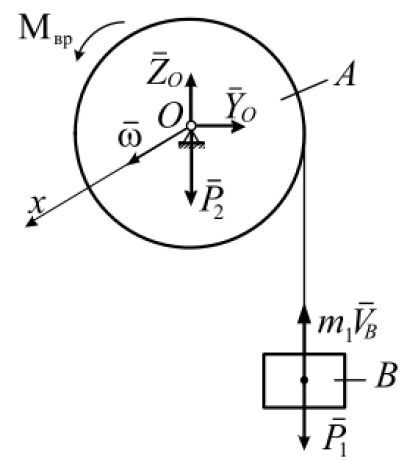
\includegraphics[height=5cm,width=1\textwidth,keepaspectratio]{image12.png}
            \label{fig:image12}
        \end{figure}
    \end{column}
\end{columns}

\end{frame}

\begin{frame}[t]{Task 2 (yours): M (rus) 37.13    }
\framesubtitle{}
    \vspace{-0.6cm}
    \begin{figure}[H]
        \centering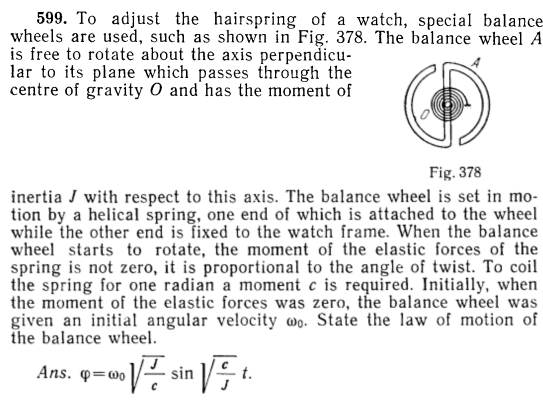
\includegraphics[height=6.5cm,width=1\textwidth,keepaspectratio]{image11.png}
        \label{fig:image11}
    \end{figure}
\end{frame}

\fbckg{fibeamer/figs/last_page.png}
\frame[plain]{}
\end{document}